\documentclass[10pt,a4paper]{article}
\usepackage[margin=1.5cm]{geometry}
\usepackage[T1]{fontenc}
\usepackage{lmodern}
\usepackage{graphicx}
\usepackage{booktabs}
\usepackage{amsmath}
\usepackage{array}
\usepackage{microtype}

\setlength{\parindent}{0pt}
\setlength{\parskip}{0.32em}
\setlength{\textfloatsep}{0.8em}
\setlength{\floatsep}{0.7em}
\renewcommand{\arraystretch}{1.13}
\newcommand{\code}[1]{\texttt{#1}}

\begin{document}

\title{Randomized Skip List: Correctness and Experimental Analysis}
\author{\textit{Anthony Iemmolo - Matricola: 304132}}
\date{27/10/2026}
\maketitle
\vspace{-2.2em}

\section*{Representation, ownership, and expected cost}
Each element is a vertical tower of nodes linked with \code{next\_r} and
\code{next\_d}.  A list has a separate sentinel at each active level.  The
sentinel key is \(\mathrm{INT64\_MIN}\), but a real data key with that same
value is valid: searches begin to the right of the sentinel.  Promotion is an
independent Bernoulli trial with \(p=1/2\), driven by the shared,
seedable \code{random\_handler}.  Thus a tower has expected height two and
the expected total number of allocated tower nodes is \(O(n)\).

\code{split} and \code{ordered\_union} move existing forward links rather
than rebuild data towers.  Their inputs remain allocated but empty and may be
used again; their outputs own the transferred nodes.  Lists sharing a handler
therefore continue one reproducible random stream.  Searching or inserting
uses the usual top-down search path, hence expected \(O(\log(n+2))\).
Structural split changes the predecessor links on that path, and ordered union
joins the two outer borders, giving expected \(O(\log(n+2))\) and
\(O(\log(n+m+2))\), respectively.  The rebuilding comparison performs an
ordinary insertion for every old key into fresh lists, so its algorithmic
expectation is \(\Theta(n\log n)\), plus linear traversal and disposal.

\section*{Correctness evidence}
The runner checks the bottom-level reference set, strictly increasing levels,
downward-level subsequences, tower heights, and ownership/reachability.  It
covers empty and singleton lists, duplicates, negative keys, both \code{int64\_t}
boundaries, and the real \(\mathrm{INT64\_MIN}\) key.  It also exercises
split--union round trips, input reuse after consumption, independent output
updates, and 1,000 mixed operations against \code{std::set}.  The checks run
with seeds \(0,7,17,27\) and are also built with AddressSanitizer and
UndefinedBehaviorSanitizer.  Structural operations additionally check that
data-node addresses and heights survive; rebuilding split instead checks for
fresh towers and the resulting random-generator state.

\section*{Benchmark method}
The measurements and figures below are taken from the saved Colab execution of
\code{google\_benchmark/notebooks/analysis\_colab.ipynb} (27 October 2026).
It used Google Benchmark 1.10.0, GCC 13.3 with \code{-O3 -DNDEBUG}, and a
2.20 GHz Intel Xeon virtual CPU.  Six sizes
\(N\in\{2^{10},2^{12},\ldots,2^{20}\}\), height seeds
\((42,900,5783)\), and three repetitions were used.

Construction, validation, and destruction are outside the timed mutation
regions.  Search times 256 shuffled queries (128 hits and 128 misses) and
insertion times 32 absent, spread-out keys; both are normalized per operation.
Union uses two ordered disjoint halves, while split uses an absent middle pivot
and balanced outputs.  Rebuilding split uses exactly the same split workload.
The raw JSON and CSV files produced by the notebook are retained under
\code{google\_benchmark/JSON/colab} and \code{google\_benchmark/CSVs/colab}.

\section*{Experimental evidence and discussion}
The relevant question is not just whether time rises with \(N\), but whether
the structural methods and the rebuilding method show the two different costs
predicted by the algorithms.  The model was chosen \emph{before} looking at the
results: Google Benchmark uses supplied \(c\log_2N\) for search, insertion,
union and structural split, and supplied \(cN\log_2N\) for rebuilding split.
No row in Table~\ref{tab:fits} is an automatically selected model.  As a
separate check, I used least squares on the same individual timings, allowing
an intercept: \(a\log_2N+b\) for the structural methods and
\(aN\log_2N+b\) for rebuilding.  The table reports the mean of the three
per-seed fits; \(R\) is normalized RMS residual.  Search and insertion
coefficients are normalized per operation.

\begin{table}[!t]
\centering
\caption{Colab CPU-time fits; each entry is the mean over seeds 42, 900, and 5783.  Log-model coefficients are in ns; the \(N\log N\) coefficients are in ns/(key\(\cdot\log_2\)key).}
\label{tab:fits}
\small
\setlength{\tabcolsep}{3.3pt}
\begin{tabular}{@{}l c r r r r r@{}}
\toprule
& supplied & \multicolumn{2}{c}{Google Benchmark} & \multicolumn{3}{c}{custom least squares}\\
Kernel & model & \(c\) & \(R\) (\%) & \(a\) & \(b\) (ns) & \(R\) (\%)\\
\midrule
search          & \(\log N\) & 20.44  & 49.35 & 51.29   & -486.75       & 30.90\\
insertion       & \(\log N\) & 220.58 & 50.32 & 614.45  & -6214.41      & 20.45\\
ordered union   & \(\log N\) & 585.78 & 41.34 & 1464.38 & -13862.41     & 16.41\\
split           & \(\log N\) & 756.07 & 49.34 & 2074.87 & -20807.70     & 19.97\\
split rebuild   & \(N\log N\) & 58.45 & 12.30 & 58.53 & -1.50\(\times10^6\) & 12.28\\
\bottomrule
\end{tabular}
\end{table}

The structural coefficients are reasonably stable across seeds: the three
Google Benchmark coefficients differ by at most about 13\% for split and less for the
other kernels.  This is expected because the seed changes tower shapes, not
the workload.  However, the no-intercept logarithmic fits have substantial
residuals (41--50\%).  Adding \(b\) lowers them to 16--31\%, which says that
fixed costs and memory effects matter over this finite range.  It does \emph{not}
prove a different asymptotic complexity: cache/TLB misses, pointer chasing,
random tower shapes, and only ten timed mutation iterations all affect time.

Rebuilding is different.  Its supplied \(N\log N\) fit has \(R=12.30\%\),
and the custom fit is almost identical (\(58.45\) versus \(58.53\) in the
coefficient and \(12.30\%\) versus \(12.28\%\) in RMS).  This is consistent
with the implementation traversing all keys and inserting each into a fresh
skip list.  In the direct comparison, rebuilding is about \(2.2\times10^2\)
times slower at \(N=1024\), growing to \(5.8\times10^4\) at \(N=2^{20}\), averaged
across seeds.  Preserving towers and rewiring a logarithmic border is therefore
not merely an asymptotic improvement; it dominates the measured cost here.
No logical-work counter was enabled, so timing alone is not evidence for the
number of links traversed.

\section*{Conclusion}
The implementation meets the intended distinction between the two approaches.
Search, insertion, ordered union, and structural split operate by following or
rewiring skip-list paths, and their measurements are consistent with slow
logarithmic growth over the tested range.  Rebuilding split instead creates new
towers through ordinary insertions, and its results are well described by the
supplied \(N\log N\) model.

The benchmark results should be read as experimental evidence rather than a
proof of complexity: measured time also includes allocation, cache behavior,
and random tower shapes.  Nevertheless, the contrast with rebuilding split is
large and stable across seeds, showing why transferring existing towers is the
right design for this operation.

\vspace{0.25em}
\begin{figure}[!b]
\centering
\begin{minipage}[t]{0.49\linewidth}
\centering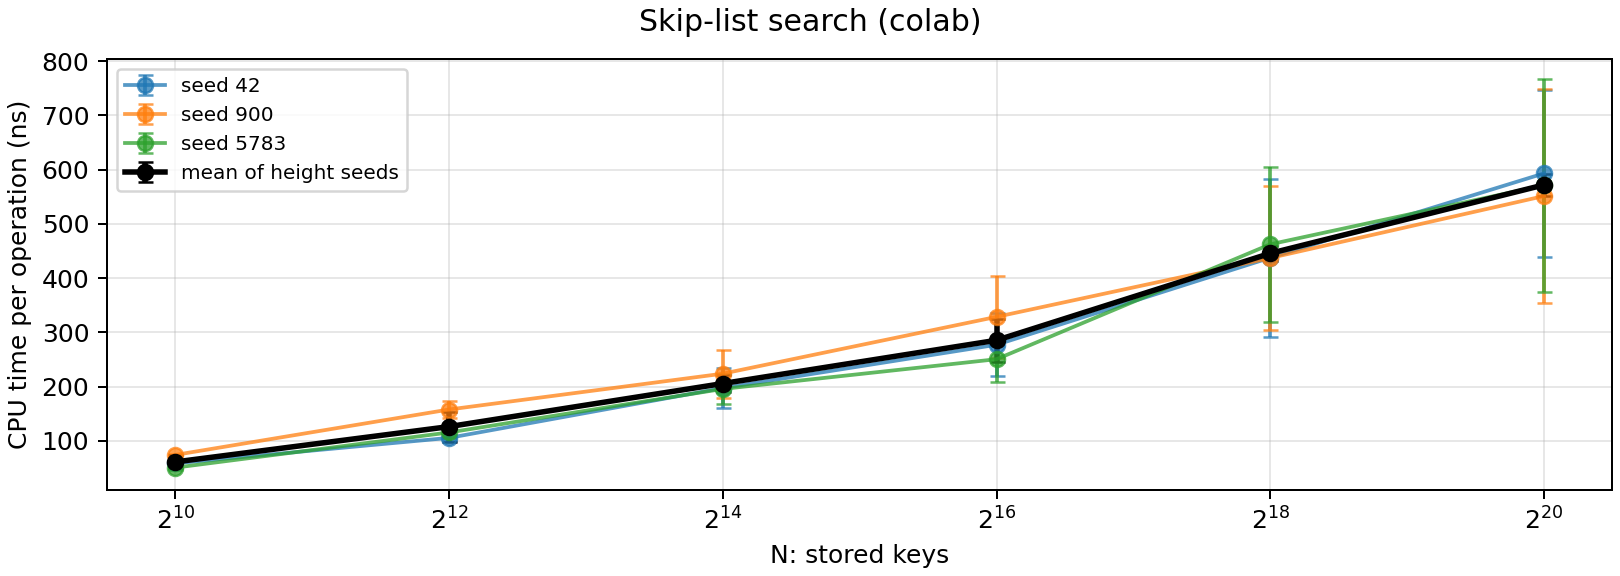
\includegraphics[width=\linewidth]{images/search.png}\\[-0.5em]
\small (a) Search
\end{minipage}\hfill
\begin{minipage}[t]{0.49\linewidth}
\centering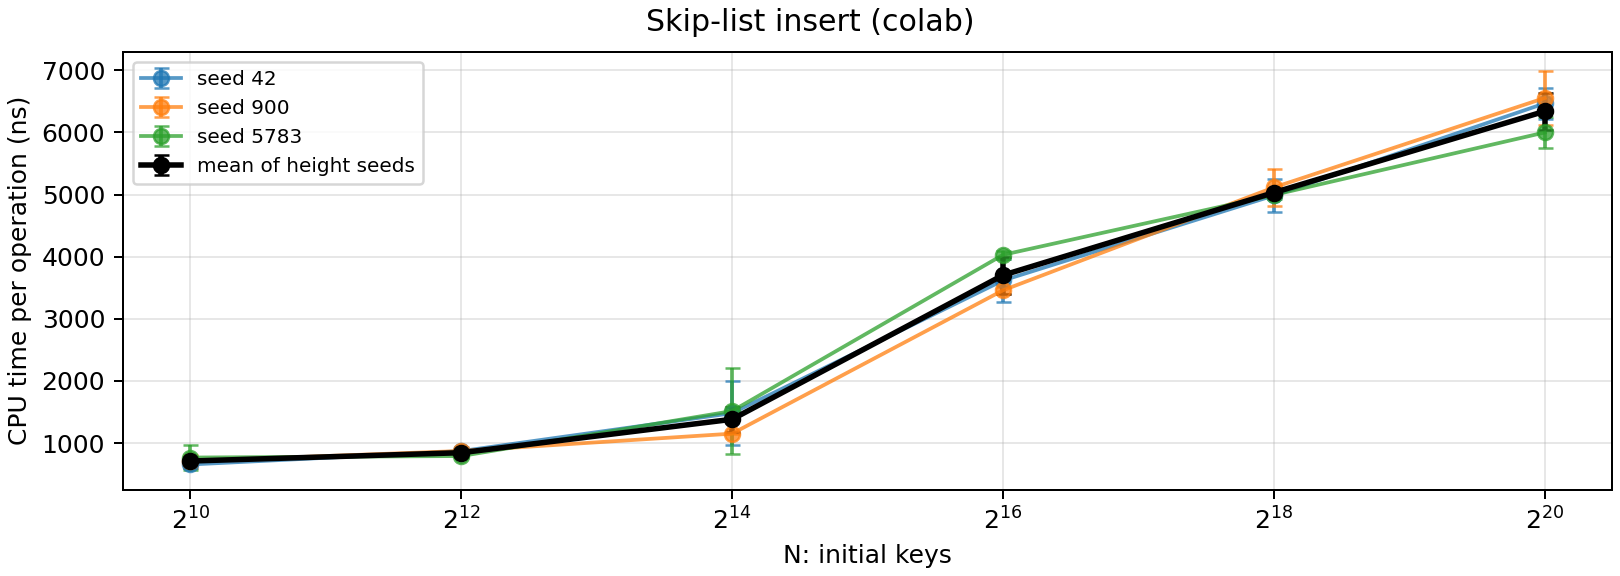
\includegraphics[width=\linewidth]{images/insertion.png}\\[-0.5em]
\small (b) Insertion
\end{minipage}

\begin{minipage}[t]{0.49\linewidth}
\centering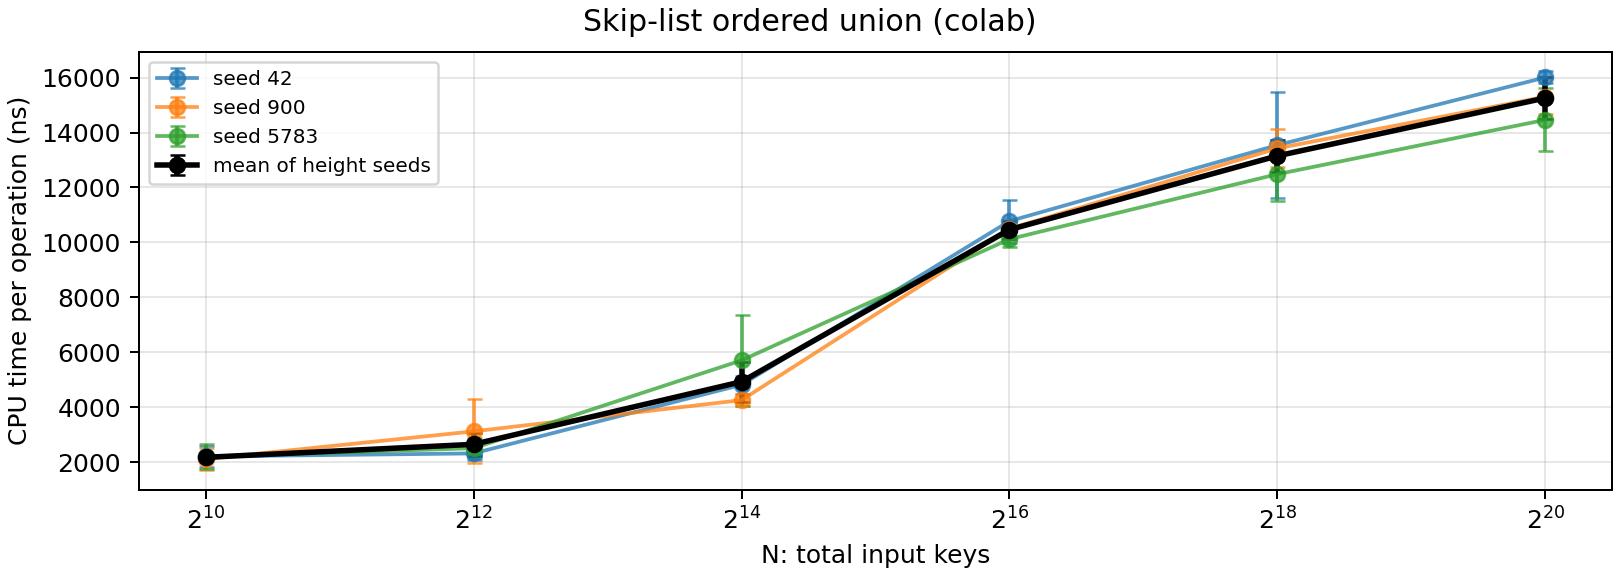
\includegraphics[width=\linewidth]{images/ordered_union.png}\\[-0.5em]
\small (c) Ordered union
\end{minipage}\hfill
\begin{minipage}[t]{0.49\linewidth}
\centering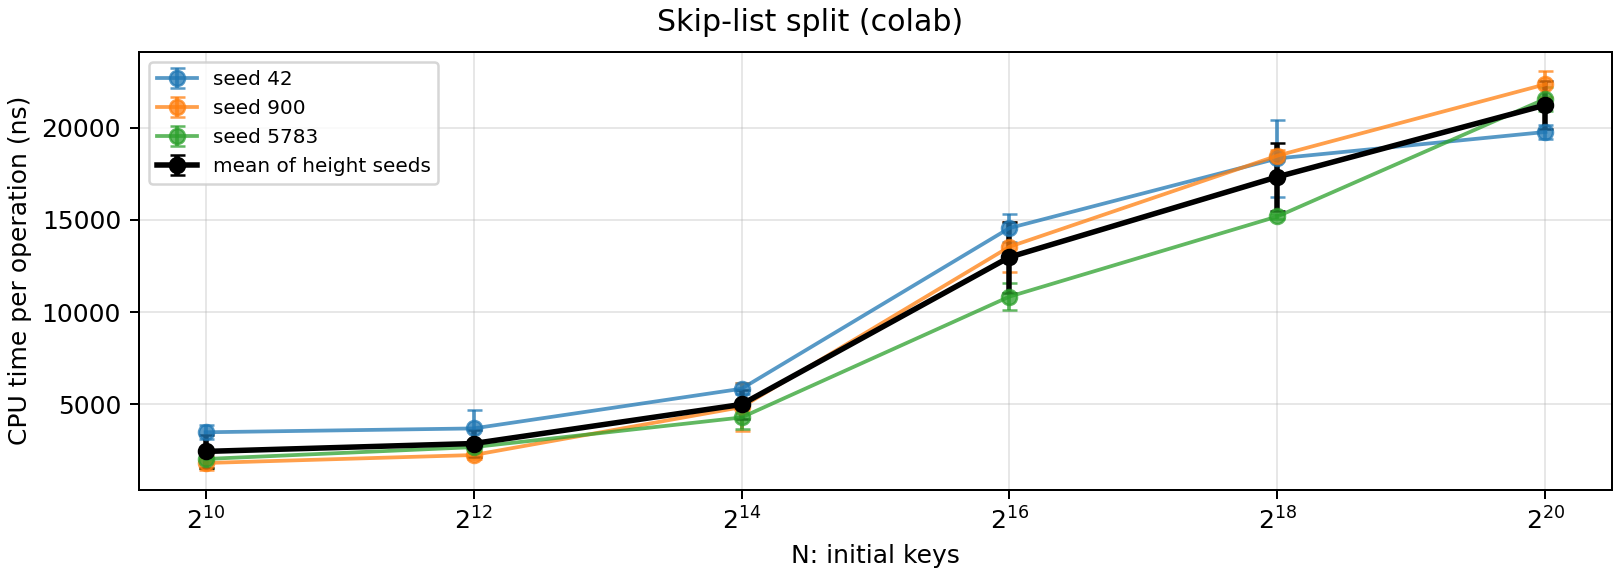
\includegraphics[width=\linewidth]{images/split.png}\\[-0.5em]
\small (d) Structural split
\end{minipage}

\vspace{0.25em}
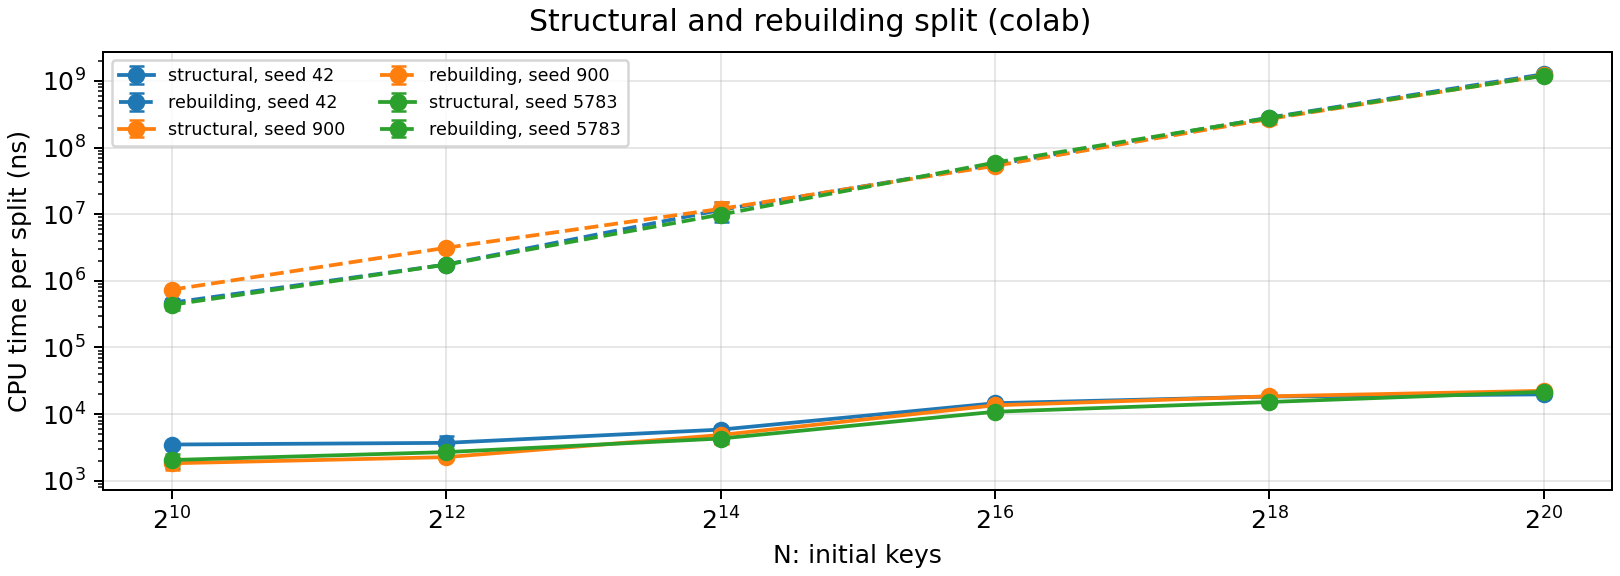
\includegraphics[width=0.75\linewidth]{images/split_comparison.png}
\caption{Figures produced by the Colab notebook from the saved raw runs.  The
top four panels show the four structural kernels; the final panel compares
structural split with rebuilding split.}
\label{fig:timings}
\end{figure}

\end{document}

